% http://mail.google.com/mail/#search/to%3Akrieger+OR+to%3Adavidahn+OR+(to%3Adavid+AND+to%3Aahn)+OR+from%3Akrieger+OR+from%3Adavidahn/120e6c9667b99ada
\documentclass[letterpaper]{article}
\usepackage{aaai}
\usepackage{graphicx}
\usepackage{times}
\usepackage{helvet}
\usepackage{courier}
\usepackage[usenames]{color}

\pdfinfo{
/Title (FIXME Formatting Instructions for Authors)
/Subject (Proceedings of the AAAI Press Conference)
/Author (AAAI)}
\setcounter{secnumdepth}{0}

% color.sty ... red green blue cyan magenta yellow

\newcommand{\bto}[1]{\textcolor{blue}{\textbf{[#1 --BTO]}}}
\newcommand{\mikeyk}[1]{\textcolor{green}{\textbf{[#1 --mikeyk]}}}

%\newcommand{\codenote}[1]{ \textcolor{cyan}{\textbf{[#1]}} }
\newcommand{\codenote}[1]{}

\newcommand{\link}[1]{\texttt{\small{#1}}}

 \begin{document}
% The file aaai.sty is the style file for AAAI Press 
% proceedings, working notes, and technical reports.
%
\title{TweetMotif: Exploratory Search and Topic Summarization for Twitter}
\author{Brendan O'Connor \\ 
Carnegie Mellon University \\ brenocon@gmail.com
\And
Michel Krieger \\ Meebo, Inc. \\ mikekrieger@gmail.com
\And
David Ahn \\ Microsoft, Inc. \\ daviddahn@gmail.com
}
\maketitle
\begin{abstract}
\begin{quote}
We present TweetMotif, an exploratory search application for Twitter.  Unlike traditional approaches to information retrieval, which present a simple list of messages, TweetMotif groups messages by frequent significant terms --- a result set's subtopics --- which facilitate navigation and drilldown through a faceted search interface.  The topic extraction system is based on syntactic filtering, language modeling, near-duplicate detection, and set cover heuristics.  We have used TweetMotif to deflate rumors, uncover scams, summarize sentiment, and track political protests in real-time.   A demo of TweetMotif, plus its source code, is available at http://tweetmotif.com.
\end{quote}
\end{abstract}

\section{Introduction and Description}

%\bto{probably need to cut this intro crap down}

On the microblogging service Twitter, users post millions of very short messages every day.  Organizing and searching through this large corpus is an exciting research problem.  Since messages are so small, we believe microblog search requires summarization across many messages at once.

\begin{figure}[htbp]
\begin{center}
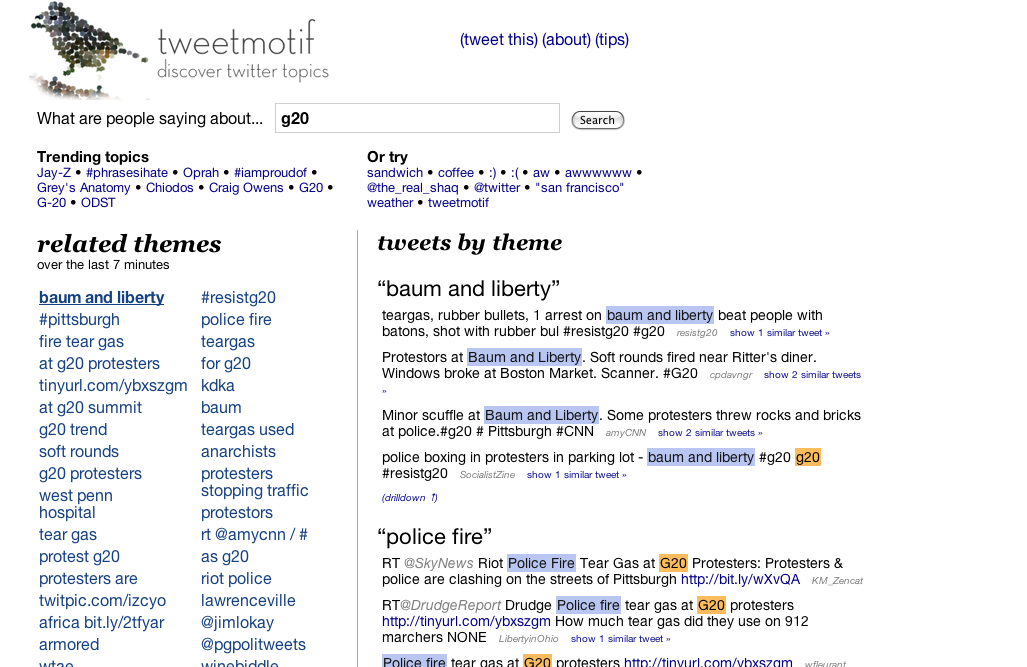
\includegraphics[scale=0.3]{screenshot.png}
\caption{Screenshot of TweetMotif.}
\label{screenshot}
\end{center}
\end{figure}

Our system, TweetMotif, responds to user queries, first retrieving several hundred recent matching messages from a simple index; we use the Twitter Search API.

Instead of simply showing this result set as a list, TweetMotif extracts a set of themes (topics) to group and summarize these messages.  A topic is simultaneously characterized by (1) a 1- to 3-word textual label, and (2) a set of messages, whose texts must all contain the label.

TweetMotif's user interface is inspired by faceted search, which has been shown to aid Web search tasks \cite{hearst_findingflow_2002}.
The main screen is a two-column layout. The left column is a list of themes that are related to the current search term, while the right column presents actual tweets, grouped by theme. As themes are selected on the left column, a sample of tweets for that theme appears at the top of the right column, pushing down (but not removing) tweet results for any previously selected related themes. This allows users to explore and compare multiple related themes at once. 

The set of topics is chosen to try to satisfy several criteria, which often conflict:

\begin{enumerate}
\item Frequency contrast: Topic label phrases should be frequent in the query subcorpus, but infrequent among general Twitter messages.  This ensures relevance to the query while eliminating overly generic terms.
\item Topic diversity: Topics should be chosen such that their messages and label phrases minimally overlap.  Overlapping topics repetitively fill the same information niche; only one should be used.
%\item Set cover: Topics should be chosen such that their message union includes as much of the query subcorpus as possible, though it is not necessary to i
\item Topic size: A topic that includes too few messages is bad; it is overly specific.
\item Small number of topics: Screen real-estate and concomitant user cognitive load are limited resources.
\end{enumerate}
The goal is to provide the user a concise summary of themes and variation in the query subcorpus, then allow the user to navigate to individual topics to see their associated messages, and allow recursive drilldown.  The approach is related to document clustering (though a message can belong to multiple topics) and text summarization (topic labels are a high-relevance subset of text across messages).  We heuristically proceed through several stages of analysis.


\subsection{Step 1: Tokenization and syntactic filtering}

Tokenization is difficult in the social media domain, and good tokenization is absolutely crucial for overall system performance.  Standard tokenizers, usually designed for newspapers or scientific publications, perform poorly.  Our regex-based tokenizer treats hashtags, @-replies, abbreviations, strings of punctuation, emoticons and unicode glyphs (e.g. musical notes) as tokens.

Unigrams are too narrow a unit of analysis; ideally, we want to extract all phrases and subphrases.  We begin with all unigrams, bigrams, and trigrams, discarding unigrams that are function words, and discarding bigrams and trigrams that cross syntactic boundaries. These rules flag n-grams including certain types of punctuation tokens in certain positions, and ones that end with certain right-binding function words like ``the'' and ``of.''  This simple syntactic filtering greatly improves the coherency of extracted n-grams.


%... hashtags get special treatment: set-like semantics, not allowed to participate in phrases

\subsection{Step 2: Score and filter topic phrase candidates}
%\cite{manning_introduction_2008}
\codenote{lang_model.py, ranking.py}
TweetMotif takes a simple language modeling approach to identifying topic phrases that are most distinctive for a tweet result set, scoring them by the likelihood ratio:
\[\frac{Pr(\textrm{ phrase } \ |\ \textrm{ tweet result set })}
{Pr(\textrm{ phrase } \ |\ \textrm{ general tweet corpus })}
\]
As is usually the case in language modeling, a given phrase does not necessarily occur in a corpus, so probabilities must be estimated with smoothing.  We tried several simple estimation methods, settling on Lidstone smoothing:
\[ Pr(\textrm{ phrase }\ |\ \textrm{corpus}) = \frac
{ \textrm{phrase count in corpus} + \delta }
{ N + \delta n }
\]
where for a phrase of length $m$, $N$ is the count of all phrase instances of length $m$ in the corpus, $\delta=0.5$ is the smoothing parameter, and $n$ is the count of all phrase types of length $m$ in the corpus.  Essentially, there are independent models for unigram, bigram, and trigram phrases.

%Since we were satisfied with Lidstone, we did not try more advanced language models like Good-Turing, Kneser-Ney, etc.
%.. interestingly, hacky MLE beat Lidstone for a while until tweaked syntactic analysis filtering \bto{explain if room}

The background corpus consists of 150,000 Twitter messages collected in April 2009 from search queries for \emph{the}, \emph{of} and several other common English function words.
%.. Backgrond corpus .. say size, admit it's tiny ..

It is interesting to compare our approach to TF/IDF for document retrieval, which estimates document relevance by balancing the frequency of query terms against their frequencies in a background corpus.  Note that the average Twitter message is 11 words long, and words rarely occur more than once in a message; thus, the count of a word is virtually the same as the count of messages it occurs in (DF and TF are the same).  If messages are considered documents, the notion of document TF is not very useful.  Our approach is more like TF for one giant document consisting of the concatenation of all query subcorpus messages.  This too is an odd analogy.  In general, we believe the microblog search problem will require creative formulations of cross-message phonemena beyond current paradigms in IR.

\subsection{Step 3: Merge similar topics}
\codenote{ deduper.py }
Every candidate phrase defines a topic, a set of messages that contain that phrase.  Many phrases, however, occur in roughly the same set of messages, thus their topics are repetitive.  We seek to merge similar topics.

First, there are easy merges between subsumed n-gram phrases of differing sizes.  Each of an n-gram's label-subsumed (n-1)-grams must conversely subsume its message set.  For example, the message set for the bigram topic ``swine flu'' must be a subset or equal to the two unigram topics ``swine'' and ``flu.''  If the ``swine flu'' topic is in fact equal to the ``flu'' topic, then we discard the ``flu'' topic, since ``swine flu'' is strictly more informative.

Furthermore, ignoring topic labels, we merge topics if their message sets have more than $90\%$ Jaccard similarity.  All pairs of topics are compared, so final topics are connected components of the pairwise $Jacc \geq 0.9$ graph --- i.e., single-link clustering.  When several topics are merged, only the intersection of messages is included in the new topic.  There is a label choice problem/opportunity for merged topics: any of the old topics' labels are now legitimate.  Our heuristic solution usually picks longer and higher scoring labels, and sometimes combines short labels into a skip n-gram.

\subsection{Step 4: Group near-duplicate messages}

\codenote{ deduper.py }
Grouping messages by topic reveals a massive amount of message duplication on Twitter.  People forward (``retweet'') interesting messages such as jokes and news headlines; 
and furthermore, a seemingly huge number of bots repeat advertisements, spam, weather reports, news feeds, other people's tweets, songs being played on personalized Internet radio stations, templated messages, etc.
It is a waste of space to always show near-duplicates to the search user; therefore we detect clusters of near-duplicates, display them with a single representative and numeric size, and allow them optionally to be viewed.  The algorithm groups messages whose sets of trigrams have a pairwise Jaccard similarity exceeding 65\%.  (For this and the topic merging step, using phrase-message indexes cuts down on the potentially quadratic runtime.)

This technique seems to reliably find retweets and other forms of repetition; it also naturally groups together spam.  This was very important in mid-2009 when we developed TweetMotif, when spam was very prevalent and retweets were not explicitly marked in the data.

\subsection{Step 5: Finalize topics}

We are now left with a ranked list of topics containing messages in near-duplicate clusters.  After eliminating topics that contain only one near-duplicate cluster, the list is cut off to the top 40 topics, and all messages that did not end up in a topic are put in a catch-all ``more...'' topic.

All the above analysis is conducted on the result set while the user waits.  A demo, examples, and source code are available at http://tweetmotif.com.

%The topic and navigation system may be compared to query refinement, which helps a user  or topic models

%Our topic-finding system bears a 


\bibliography{tweetmotif.bib}
\bibliographystyle{aaai}


\end{document}
